\subsection{Concept Clustering}
To identify multiple senses of a term automatically, we first use a k-Medoids clustering algorithm on the concept context of the term, and then
we select the center concept in each cluster to represent a sense of this term.  Figure~\ref{fig:clustersOfApp}(a) shows the concept context of
the term ``apple'', and Figure~\ref{fig:clustersOfApp}(b) shows the clustered concepts. It is clear that each cluster represents a sense of the
term.

\begin{figure}[!h]
 \centering
 \includegraphics[width=0.98\columnwidth]{clusteringResultShow.eps}
 \caption{The concept context of ``apple''}
 \label{fig:clustersOfApp}
\end{figure}

In the following, we define the distance measure and present the
clustering algorithm.

%\subsubsection{Distance Measure}

%We first introduce the lexical distance measure to identify those terms with very similar surface forms caused by the misspelling, for example, .... In terms of the edit-distance, we merge these similar concepts with a representative one and combine their entity distributions. After this preprocessing, we use the semantic distance measure function defined in \ref{eq:semanticDist} to evaluate the distance between concepts.

\subsubsection{Clustering Algorithm}
We first define the semantic distance between two concepts $c_1$ and
$c_2$ as
\begin{equation}
\label{eq:semanticDist}
\begin{aligned}
d_{sem}(c_{1}, c_{2}) = 1-cosine(\mathcal{I}_{c_{1}}, \mathcal{I}_{c_{2}})
\end{aligned}
\end{equation}
where $\mathcal{I}_{c_i}$ represents the vector of entity distributions
of concept $c_i$ as defined in \eqnref{eq:Ic}.

Our algorithm is a modified k-Medoids clustering algorithm that partitions concepts according to their entity distributions. Good initial
centers are essential for the success of partitioning clustering algorithms such as K-Medoids. Instead of using random initial centers, we
identify good initial centers incrementally by a refined method from
Moore \cite{Moore:1991}. %\KZ{How is the $\alpha$
%related to $K$? Please don't expect the reader to read the Moore paper to find out what's $\alpha$.}
The first medoid is randomly selected among all candidate points
(concepts). Then we select the point that has the maximum of the
minimum of the distances from each of the existing medoids to be the
next medoid, i.e.,
\begin{equation}
m = \{m_i|\max_{c_j}\{\min_{i}\{d_{sem}(m_i,c_j)\} \} > \alpha\}\label{eq:initMedoid}
\end{equation}
where $c_j$ indicates the $j^{th}$ point in the candidate points,
$m_i$ indicates the $i^{th}$ medoid in existing medoids, and $\alpha$ indicates the threshold in the limit of initial medoid count.
%Then, the point that
%has the maximum distance to existing medoids % (defined by the minimum
%% distance to any of the existing medoid)
%is selected to be the next medoid.
This process continues until we do not find any medoids satisfying \eqnref{eq:initMedoid}.
%have chosen $k$ medoids%
In this case, we get $k$ medoids at iteration 0: $M^{0} = \{m_{1}^{0}, ..., m_{k}^{0}\}$. Clearly, the value of $k$ is determined by the
threshold $\alpha$. The larger the threshold of $\alpha$, the small the value of $k$. Since experiments show that the numbers of clusters do not
vary much with $\alpha$ between 0.7 to 0.8, we set $\alpha$ = 0.7 as an optimal value.

%How to update after once iteration (how to determine the centroid)?
With \emph{k} medoids in the $t^{th}$ iteration, we assign each
candidate concept $c_{i} \in C$ to its closest medoid $m^{*}\in M^{t}
= \{m_{1}^{t}, ..., m_{k}^{t}\}$, namely, a medoid $m^{*}$ with the
minimum semantic distance from $c_{i}$:
\begin{equation}
\label{eq:newCentroid}
m^* = \argmin_{m_{j}^{t}\in M^{t}}d_{sem}(c_{i}, m_{j}^{t})
\end{equation}
When we assign all candidate concepts to the corresponding clusters,
we can update the medoid with the most centrally located concept in
each cluster.  To find such a center concept, we first compute the
average distance of a cluster $K_{i}$ in terms of the semantic
distance in \eqnref{eq:semanticDist} as
\begin{equation}
\label{eq:update}
m_i^{t+1} = \argmin_{c_{y}\in K_{i}}\left(\sum_{c_x\in K_{i}}\frac{d_{sem}(c_{x},c_y)}{|K_{i}|}\right)
\end{equation}
%Thus, we find the new centroid $m^{t+1}_{i}$ in the $(t + 1)^{th}$ iteration
%whose the average semantic distance is the minimum one.
The clustering process iterates until the following objective function reaches
minimum.
%What should be the objective function of clustering?
%The objective function is to find \emph{W} and \emph{M} that minimize
\begin{equation}
\label{eq:objectiveFun}
\begin{aligned}
F(W,M)=\sum^{k}_{i=1}\sum^{n}_{j=1}w_{ij}d_{sem}(m_{i},c_{j})
\end{aligned}
\end{equation}
where \textit{w}$_{ij}\in$\{0, 1\},
$\sum^{k}_{i=1}w_{ij}=1$, 0$<\sum^{n}_{j=1}w_{ij}<n$,
$k~ (<n)$ is a known number of centers, \emph{n} is the count of objects (concepts) to cluster.
$W = [w_{ij}]$ is a
$k \times n$ binary matrix, $M=[m_{1}, \ldots, m_{k}]$ is a set of cluster medoids
and $m_i$ is the $i^{th}$ cluster medoid.

%The matrices \emph{W} and \emph{M} are calculated according to the following two theorems provided in \cite{Ng:2007}.
We use \eqnref{eq:update} to calculate the medoid set $M$.
When $M$ is computed, to minimize $F(W, M)$, $W$ is given by
\begin{equation}
\label{eq:weight}
\noindent {w_{ij} = \left\{
\begin{aligned}
1 & \hspace*{5pt} \mbox{if}~ d_{sem}(m_{i},c_{j}) < d_{sem}(m_{h},c_{j})\\
 & \hspace*{25pt} (1 \leq h \leq k,~h \neq i)\\
0 & \hspace*{5pt} \mbox{otherwise}
\end{aligned}
\right.}
\end{equation}
The convergence condition is that $F(W^{t}, M^{t+1})- F(W^{t}, M^{t})$
is less than a threshold $\delta$ (e.g., $10^{-5}$).
According to the above processing of k-Medoids, we can get \emph{k} clusters for all given concepts.
%The minimization
%of \emph{F} with the above constraints is an undecidable constrained nonlinear
%optimization problem. A partial optimization for $M$ and $W$ is
%shown in Algorithm \ref{alg:conceptClustering}.

%%\makeatletter\def\@captype{algorithm}\makeatother
%\renewcommand\algorithmicrequire{\textbf{Input:}}
%\renewcommand\algorithmicensure {\textbf{Output:}}
%\begin{algorithm}[th]
%%\begin{center}
%\caption{Concept Clustering}
%\label{alg:conceptClustering}
%%\caption{Context-based semantic cleaning approach} \label{algo_minball}
%\begin{algorithmic}[1]
%\REQUIRE $C=\{c_{1}, ...c_{j},...\}$: the concept set;\\
%~~~~~~~$\alpha$: the threshold in the limit of initial medoid count;\\
%~~~~~~$T$: the maximum iteration count; \\
%~~~~~~$\Gamma_{isA}$: the semantic network of isA relationship;\\
%\ENSURE \emph{k} clusters $\{K_{1}, ..., K_{k}\}$; \STATE Initialize the iteration time \emph{t} = 0; \STATE Generate an initial medoid set
%$M^{t}=[m_{1}^{t}, m_{2}^{t}, \cdots, m_{k}^{t}]$ incrementally by Eq.~\ref{eq:initMedoid}; \STATE Assign each concept $c_{i}$ to a cluster
%$K^{*}$ with a medoid $m^{*}$ satisfying \eqnref{eq:newCentroid}; \STATE Update the weight matrix $W^{t}$ in \eqnref{eq:weight} to make sure
%$F(W^t, M^t)$ is minimum; \STATE Update cluster medoids in $M^{t+1}$ with the most centrally located point in each cluster corresponding to
%\eqnref{eq:update}; \STATE Calculate $F(W^t, M^{t+1})$ in \eqnref{eq:objectiveFun}; \IF {$F(W^t, M^{t+1})$-$F(W^t, M^t)$ $ > \delta$ and
%\emph{t} < \emph{T}} \STATE Let \emph{t} = \emph{t}+1 and go to Step 3; \ENDIF \STATE return clusters $\{K_{1}, ..., K_{k}\}$;
%\end{algorithmic}
%%\end{center}
%\end{algorithm}

\subsubsection{Offline Concept Clustering}
%We first analyze the computational complexity in our concept clustering approach.
The k-Medoids clustering algorithm has a time complexity of $O(kn^{2})$,
where $k$ is the number of centers and $n$ is the number of objects (concepts)
to cluster.
%In this case, given a pair of terms, if we install clustering after we collect the concept contexts (we call this processing as the online clustering), it is hard to apply into measuring the semantic similarity of millions pairs even if online clustering for each pair consumes only a few seconds. More precisely, suppose we have 1 million pairs and the time overhead of online clustering for each pair is only 1 second, we will spend 11.57 days at least on the measuring of semantic similarity of all pairs.
This is not acceptable if the number of pairs is large.
To improve the efficiency, we cluster all concepts
in the semantic network offline, and then during online calculation,
each concept in a term's context can be quickly mapped to an offline cluster
which acts as synset, and this effectively reduces the online clustering
complexity to $O(n)$.
%we only need to find the cluster information directly after collecting
%the concept contexts of a pair.
%In this case, the time overhead of clustering the concept context
%of each term can be reduced to 5 milliseconds on average.
%We call this processing as the offline clustering.

\begin{figure}[th]
%\makeatletter\def\@captype{figure}\makeatother
 \centerline{
 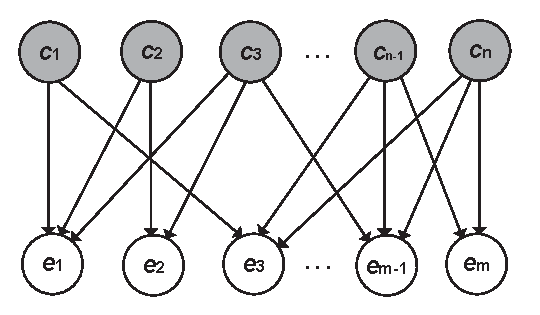
\includegraphics[width=0.9\columnwidth]{bipartition-small.eps}}
\caption{A concept-entity bipartite graph} \label{fig:bipartition}
\end{figure}

%There are some challenges in the clustering all concepts
%in the semantic network.
To cluster the concepts in the semantic network, we use the entity distributions to represent the concepts and evaluate their similarities by \eqnref{eq:semanticDist}. According to the isA relationships between concepts and entities in $\Gamma_{isA}$, we can construct a bipartite graph
between concepts and entities (Figure~\ref{fig:bipartition}) and cluster the concepts based on this graph. The basic idea is that if two
concepts share many entities, they are similar to each other. From this bipartite graph, we represent each concept $c_i$ as an L2-normalized
vector as shown in \eqnref{eq:Ic}, where each dimension corresponds to an entity in the graph.

Even though the number of concept and entity nodes may be large,
%On the surface, there are two challenges in clustering concepts
%on the bipartite graph. First, the concept nodes in this bipartite are large,
%as $\Gamma_{isA}$ consists of more than 2.7 million unique concepts.
%Therefore, the clustering algorithm must be efficient and scalable
%to handle large data sets.
%Second, the dimension $\mathcal{I}_c$ is also large, with
%over 5.5 million unique entities in $\Gamma_{isA}$.
%the data set is hence of extremely high dimensionality.
%Therefore, the clustering algorithm must tackle the
%``curse of dimensionality''.
the graph is actually very sparse.
%To overcome the above problems and find the closest cluster fast in our algorithm, we observe that the concepts in $\Gamma_{isA}$ are very sparse.
For example, a concept is connected with an average
number of 5.72 entities in $\Gamma_{isA}$. Each entity is also connected to a couple of concepts on average.
%The average degree of entities nodes is only 2.58.
Therefore, for a concept $c$, the average size of $S_c$,
the set of concepts which share at least
one entity with $c$, is small.
%is only $5.72\times (2.58-1) = 9.04$. Intuitively,
%for any cluster $C$, if $C \cap S_c = \emptyset$, \emph{C} cannot be close to $c$ since the distance of any member of \emph{C} to $c$ is 1, which is the farthest distance calculated according to \eqnref{eq:semanticDist}.
To find the closest cluster to $c$,
we only need to check the clusters which contain at
least one concept in $S_c$. Since each concept belongs to only one
cluster in our method, the average number of clusters to be checked is small.
%no more than 9.04.
%We thus use an efficient dimension array data structure\cite{Cao:2008}
%to facilitate the above checks.
Furthermore, edges in the graph with low weights (i.e., low typicality scores)
are likely to be noises and can be ignored.
%This can further simplify the graph and speed up the clustering.
%be formed due to some noisy isA relationships especially for lower co-occurrences of concepts and entities. Thus, we aim to prune these noisy concepts and entities without degrading the quality of clusters. More precisely, let $w_{ij}$ be the weight (namely the typicality score $p(e_j|c_i)$) between $c_i$ and $e_j$, let $w_i$ be the sum
%of the weights of all entities that $c_i$ contains, i.e.,
%$w_i =\sum_j w_{ij}$. We can prune an edge connecting $c_i$ and $e_j$ if the absolute
%weight the relative weight $w_{ij}/w_i < \alpha$, in our experiments,
%we set $\alpha =$ 0.001.
%After the pruning process, our clustering algorithm can finish in 15 hours when clustering 2.7 million concepts in $\Gamma_{isA}$ running on a PC of 4 GB main memory.
%


%%% Local Variables:
%%% mode: latex
%%% TeX-master: "paper"
%%% End:
